% Version 2020
% Capítulo 9. Síntesis de las comunicaciones de a bordo

% 9.1 Comunicaciones en VHF
% 9.2 Comunicaciones en HF

\chapter{S\'intesis de comunicaciones a bordo}
\label{chap:09.sintesis.comunicaciones.a.bordo}


\section{Introducci\'on}
\label{sec:09.00.introduccion}


Con el correr del tiempo se desarrollaron medios de comunicaci\'on utilizando las ondas electromagn\'eticas, con lo cual se logr\'o la transmisi\'on de gran cantidad de informaci\'on a los pilotos, las cuales no consisten s\'olo en comunicaci\'on verbal sino tambi\'en datos necesarios para la seguridad del vuelo.

Hoy en d\'ia resulta dif\'icil imaginar una aeronave, independiente de su tama\~no, sin un sistema de comunicaciones a bordo. A\'un las m\'as peque\~nas pueden contar con un simple transmisor-receptor de radio para sus comunicaciones con tierra, ver Figura \ref{fig:U09.esquema.comunicaciones.actual}.

\begin{figure}[!ht]
  \centering
   \includegraphics[width=\textwidth]{09.sintesis.comunicaciones.a.bordo/Imagenes.U09/comunicaciones.gif}
  \caption{Esquema de comunicaciones actuales}
  \label{fig:U09.esquema.comunicaciones.actual}
\end{figure}

El gran desarrollo tecnol\'ogico de la \'epoca ha hecho posible disponer de equipos de radio aeron\'auticas de diversos tipos, tama\~nos reducidos y gran variedad de posibilidades. 

Los equipos de radios pueden transmitir desde la voz hasta datos y, tambi\'en, modificar de forma aleatoria las frecuencias de emisi\'on (Have Quick), codificando sus transmisiones con claves secretas de forma que s\'olo los equipos que disponen de las mismas puedan comunicarse.



Un equipo de radio a bordo de la aeronave tiene como funci\'on principal comunicarse con los controles de tr\'afico a\'ereo que se encuentran en tierra, \ac{ATC}, 
de forma de proveer un flujo de aeronaves controlado en las operaciones de decolaje y aterrizaje en los aer\'odromos. 

El esquema b\'asico de un sistema de comunicaciones por voz se muestra en la Figura \ref{fig:sistema.radio.x.voz}.

\begin{figure}[!h]
  \centering
  \subfigure[ Emisor de amplitud modulada]{
	\includegraphics[height=6cm]{09.sintesis.comunicaciones.a.bordo/Imagenes.U09/emisor-am.gif}
	}
  \subfigure[ Receptor de amplitud modulada]{
	\includegraphics[height=6cm]{09.sintesis.comunicaciones.a.bordo/Imagenes.U09/receptor-am.gif}
	}
  \caption{Sistema de radio por voz}
  \label{fig:sistema.radio.x.voz}
\end{figure}



%\section{Introducci\'on}
\label{sec:comunicaciones.a.bordo.introduccion}

Hubo \'epocas en la aviaci\'on en las cuales los pilotos se encontraban volando solos, librados a su suerte, sin posibilidad de comunicarse con otros que se encontraban en tierra o en vuelo.

Con el correr del tiempo se desarrollaron medios de comunicaci\'on utilizando las ondas electromagn\'eticas, con lo cual se logr\'o la transmisi\'on de gran cantidad de informaci\'on a los pilotos, las cuales no consisten s\'olo en comunicaci\'on verbal sino tambi\'en datos necesarios para la seguridad del vuelo.

Hoy en d\'ia resulta dif\'icil imaginar una aeronave, independiente de su tama\~no, sin un sistema de comunicaciones a bordo. A\'un las m\'as peque\~nas pueden contar con un simple transmisor-receptor de radio para sus comunicaciones con tierra, ver Figura \ref{fig:U09.esquema.comunicaciones.actual}.

\begin{figure}[!h]
  \centering
   \includegraphics[width=\textwidth]{Imagenes.U09/comunicaciones.gif}
  \caption{Esquema de comunicaciones actuales}
  \label{fig:U09.esquema.comunicaciones.actual}
\end{figure}

El gran desarrollo tecnol\'ogico de la \'epoca ha hecho posible disponer de equipos de radio aeron\'auticas de diversos tipos, tama\~nos reducidos y gran variedad de posibilidades. 

Los equipos de radios pueden transmitir desde la voz hasta datos y, tambi\'en, modificar de forma aleatoria las frecuencias de emisi\'on (Have Quick), codificando sus transmisiones con claves secretas de forma que s\'olo los equipos que disponen de las mismas puedan comunicarse.


Un equipo de radio a bordo de la aeronave tiene como funci\'on principal comunicarse con los controles de tr\'afico a\'ereo que se encuentran en tierra, \acronimo{ATC}, de forma de proveer un flujo de aeronaves controlado en las operaciones de decolaje y aterrizaje en los aer\'odromos. 

El esquema b\'asico de un sistema de comunicaciones por voz se muestra en la Figura \ref{fig:sistema.radio.x.voz}.

\begin{figure}[!h]
  \centering
  \subfigure[ Emisor de amplitud modulada]{
	\includegraphics[height=6cm]{Imagenes.U09/emisor-am.gif}
	}
  \subfigure[ Receptor de amplitud modulada]{
	\includegraphics[height=6cm]{Imagenes.U09/receptor-am.gif}
	}
  \caption{Sistema de radio por voz}
  \label{fig:sistema.radio.x.voz}
\end{figure}


\section{Espectro de frecuencias}
\label{sec:comunicaciones.a.bordo.espectro.frecuencias}

El espectro radioeléctrico es parte del espectro electromagnético, no se ve, no se siente, pero está presente en nuestra vida diaria, cuando escuchamos la radio, cuando vemos noticias o un partido de fútbol en la televisión, cuando usamos el Wi-Fi de nuestras casas para conectarnos a Internet, cuando hablamos por teléfono celular, usamos WhatsApp, cuando viajamos por avión o conectamos nuestros dispositivos inalámbricos en el vehículo. En este sentido, el medio o la autopista que hace posible toda esta comunicación se conoce como espectro radioeléctrico, es uno de los activos intangibles más preciados de cada país, su correcta gestión impacta el PIB, el desarrollo de nuestros países y el despliegue de Internet para conectar a toda la población.

El espectro radioeléctrico entonces, es la autopista por la que viajan todas las señales que nos comunican a través del espacio libre. La luz es una onda electromagnética que podemos ver, por lo que los principios físicos que se aplican a la óptica son los mismos de las ondas electromagnéticas, la diferencia con la luz es que las ondas de radio no las puede ver ni sentir el ser humano. Para lograr usar el espectro radioeléctrico en las comunicaciones, hay que usar tecnología especial que permita identificarlas y con ello administrarlas.

La ciencia que se ocupa de estudiar el comportamiento de las ondas de radio se conoce como electromagnetismo. En 1873 el Inglés James Clark Maxwell presenta la teoría unificada de la electricidad y el magnetismo fundando la ciencia del Electromagnetismo, fue este trabajo el que preparó el escenario para todos los grandes logros en física, telecomunicaciones e ingeniería eléctrica que iban a seguir. En ella postula que la luz está compuesta por ondas electromagnéticas, pero que pueden existir ondas electromagnéticas en frecuencias distintas a las de la luz. 15 años después el científico alemán Rudolf Hertz comprueba la teoría planteada por Maxwell y publica su trabajo sobre ondas eléctricas en 1893, logrando fabricar el primer transmisor y receptor que se conoce, estos experimentos fueron conocidos por el empresario y científico Italiano Guillermo Marconi quien desarrolla antenas, transmisores y receptores básicos para lograr transmitir información a través del aire utilizando el código Morse, finalmente encuentra apoyo en el gobierno inglés para construir la primera estación de radio a gran escala y con ello logra comunicación a través del canal de la mancha y posteriormente, en los albores del siglo XIX, logra la primer comunicación transoceánica entre la estación de Poldhu y la estación de San Jhones en Newfoundland en Canadá, en el año 1901.

A partir de ese momento la humanidad entró en una nueva era, ya que la comunicación entre continentes se volvió inmediata y el transporte marítimo entre América y Europa, cuyos barcos se mantenían incomunicados varios meses en los que no se sabía de su destino, finalmente, podían comunicarse con las estaciones costeras utilizando radiocomunicaciones.

El Titanic y su hundimiento dieron pautas importantes en la forma de organizar a nivel mundial el uso de las radiocomunicaciones. Cuando el Titanic envío por radio señales de auxilio, estas fueron recibidas por varios receptores alrededor del mundo y todos ellos retransmiten información a la base de Nueva York donde se suponía que tenía que llegar el barco, pero era tanta la confusión por información tan variada que llegaba de diferentes sitios, que fue necesario ir hasta el sitio del hundimiento para saber exactamente qué había pasado.

Para que esto no volviera a suceder los países del mundo se pusieron de acuerdo para coordinar el uso del espectro radioeléctrico, dando nacimiento a lo que hoy en día se conoce como la Unión Internacional de Telecomunicaciones (UIT), el organismo especializado de las Naciones Unidas en telecomunicaciones y radiocomunicaciones, responsable de la coordinación del uso del espectro radioeléctrico así como de las órbitas satelitales.

El objetivo de la ingeniería de radiocomunicaciones es enviar la máxima cantidad de información utilizando el menor espectro posible, diseñando antenas, transmisores y receptores y lo que se conoce como esquemas de modulación, que han permitido lograr tal propósito. Uno de los últimos casos que vale la pena resaltar es la televisión digital, lo cual significó poder enviar varios canales digitales utilizando un solo canal analógico. Gracias a su novedoso esquema de modulación, con esta innovación, se liberó una porción importante del espectro para que pudiera ser utilizada por servicios que demandan intensivamente espectro como la telefonía móvil celular (servicios IMT), proceso que se conoció a nivel mundial como el dividendo digital. Las radiocomunicaciones no reconocen fronteras políticas, por consiguiente se propagan por grandes extensiones de territorio, principalmente en las zonas de frontera, por ello es importante llevar a cabo coordinaciones que permitan una utilización armoniosa del espectro.

Cada 4 años se reúnen en Ginebra Suiza por un mes, las máximas autoridades en radiocomunicaciones de más de 193 países de América, Europa, Asia, Rusia, China, la India, África y los Países árabes, en lo que se conoce como la Conferencia Mundial de Radiocomunicaciones (CMR), en dicha conferencia se analiza en consenso cómo se va a atribuir el espectro radioeléctrico, es decir cómo se van a redistribuir porciones del espectro a los diferentes servicios de radiocomunicaciones, y se aceptan nuevos estándares y tecnologías. Estos consensos son importantes porque permiten que exista la armonización en el uso del espectro, y con ello aprovechar las economías de escala. Para dar un ejemplo, observemos como nuestro teléfono celular funciona correctamente en América, Europa o el resto del mundo, esto obedece a que en las CMR todos los países se han puesto de acuerdo en las bandas que serán utilizadas por el servicio de telefonía móvil celular, así un fabricante puede producir los dispositivos móviles a escala mundial con un impacto en costos bajos debido a las economías de escala que se logran.


\begin{figure}[!htb]
  \centering
  \subfigure[La estación de Poldhu en Cornwall Inglaterra, torres de madera de 70 metros de altura y un transmisor con potencia de 25000 vatios.]{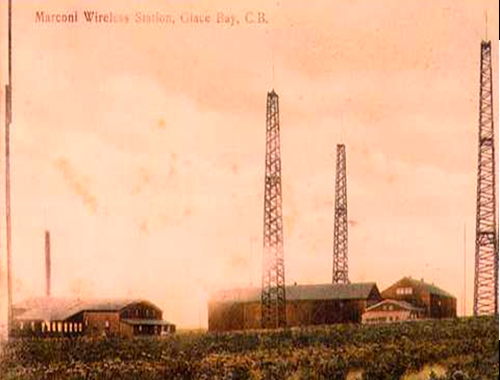
\includegraphics[width=0.40\textwidth]{09.sintesis.comunicaciones.a.bordo/Imagenes.U09/U09_estacion_cornwall_original.jpg}} \hspace{3mm}
\subfigure[Monumento en Saint Jhones, Newfoundland Canada, donde se recibió la primer comunicación interoceánica desde la estación de Pholdu.]{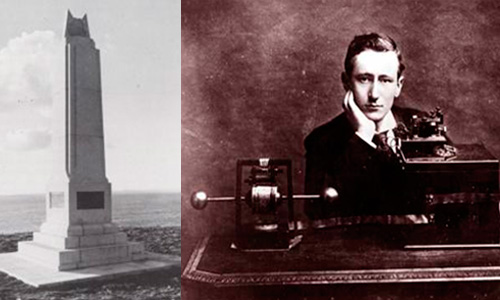
\includegraphics[width=0.50\textwidth]{09.sintesis.comunicaciones.a.bordo/Imagenes.U09/U09_Monumento-en-Saint-Jhones-Newfoundland-Canada.jpg}}

  \caption{Im\'agenes hist\'oricas de radiocomunicaci\'on. Fuente \protect\cite{historia_radiofrecuencias}}
  \label{fig:09.imagenes.historicas.radiocomunicacion}
\end{figure}


El espectro radioel\'etrico es el subconjunto de las ondas electromagn\'eticas comprendidas entre las frecuencias de 
9 kHz y 30 GHz.

Dichas frecuencias soportan una amplia gama de aplicaci\'on para negocios, usos personales, industriales, cient\'ificos,
m\'edicos y culturales, tanto p\'ublicos como privados.


%\gloss{VHF}

\begin{figure}[!htb]
  \centering
 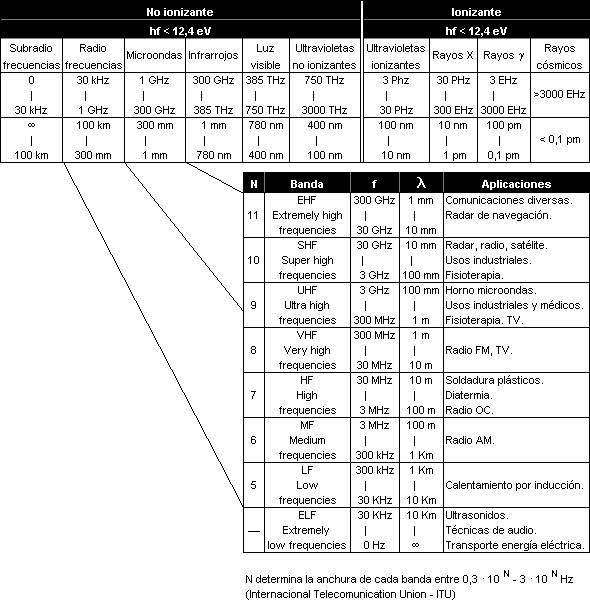
\includegraphics[width=0.9\textwidth]{09.sintesis.comunicaciones.a.bordo/Imagenes.U09/espectro-frecuencias.jpg} 
  \caption{Espectro de frecuencias, Referencia \protect\cite{Espectro_comunicaciones}}
  \label{fig:espectro.frecuencias}
\end{figure}



\section{Transceptor}
\label{sec:09.01.transceptor}

\subsection{Un sistema simple de radio}
\label{sec:09.01.01.sistema.simple.radio}


La Figura \ref{fig:09.sistema.simple.radio}  muestra un sistema de comunicación por radio de Onda Continua (en inglés Continuos Wave, CW) que comprende un transmisor y un receptor para usar con señales de onda continua (CW). La comunicación se logra simplemente activando o desactivando la señal de radiofrecuencia. La codificación se puede lograr interrumpiendo el suministro a la etapa del amplificador de potencia o incluso a la etapa del oscilador; sin embargo, normalmente se aplica dentro de la etapa del conductor que opera a un nivel de potencia más modesto. La codificación de la etapa del oscilador generalmente da como resultado una estabilidad de frecuencia deteriorada. Por otro lado, intentar interrumpir las corrientes y/o voltajes apreciables que aparecen en la etapa del amplificador de potencia también puede resultar algo problemático.

La forma más simple de receptor CW consiste en nada más que un amplificador de radiofrecuencia (que proporciona ganancia y selectividad) seguido de un detector y un amplificador de audio. La etapa del detector mezcla una señal de radiofrecuencia generada localmente producida por el oscilador de frecuencia de latido (BFO) con la señal entrante para producir una señal que se encuentra dentro del rango de frecuencia de audio (típicamente entre 300 Hz y 3.4 kHz).

Como ejemplo, suponga que la señal entrante está a una frecuencia de 100 kHz y que el BFO 
está produciendo una señal a 99 kHz. Aparecerá una señal en la diferencia entre estas dos frecuencias (1 kHz) en la salida de la etapa del detector. Esto se amplificará dentro de la etapa de audio antes de ser alimentado al altavoz.


\begin{figure}[!htb]
  \centering
  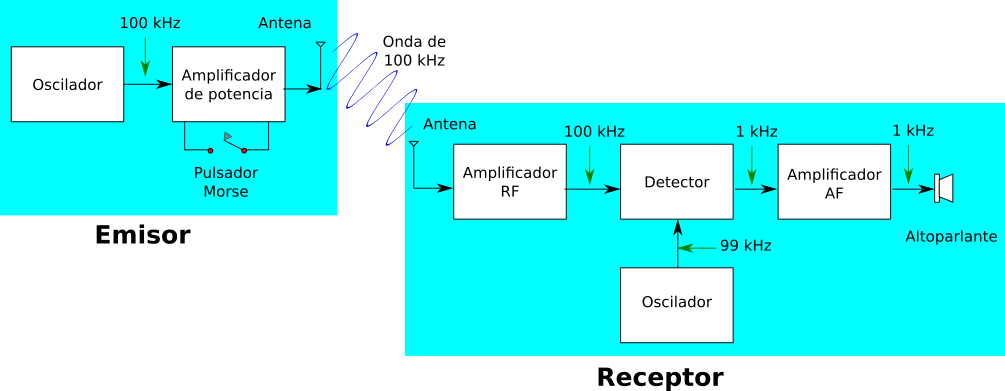
\includegraphics[width=\textwidth]{09.sintesis.comunicaciones.a.bordo/Imagenes.U09/U09_receptor_simple_radio.png}
  \caption{Sistema simple de radio para comunicaci\'on, adaptado de \protect\cite{Tooley_Aircraft_communications_and_navigation_systems}}
  \label{fig:09.sistema.simple.radio}
\end{figure}


% Ejemplo 3.1.1

% Una onda de radio tiene una frecuencia de 162. 5 kHz. Si se va a obtener una frecuencia de tiempo de 1,25 kHz, determine las dos posibles frecuencias de BFO.


% El BFO puede ser superior o inferior a la frecuencia de la señal entrante en una cantidad que es igual a la frecuencia del latido (es decir, la señal audible que resulta del 'latido' de las dos frecuencias y que aparece en la salida de la etapa del detector).

% % Por lo tanto,] sFO u003d! RF Â ±] AF desde el cual:

% % fsFO u003d (1 62.5 ± 1 .25) kHz u003d 1 60.75 o 1 63 .25 kHz

% Pon a prueba tu comprensión 3.1

% Se produce una señal de frecuencia de audio de 850 Hz cuando un BFO se establece en 455.5 kHz. ¿Cuál es la frecuencia de la señal de entrada al detector?





\subsection{Transmisor}
\label{sec:09.01.02.transmisor}


\begin{figure}[!htb]
  \centering
  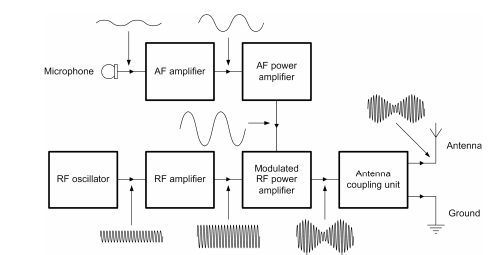
\includegraphics[width=0.75\textwidth]{09.sintesis.comunicaciones.a.bordo/Imagenes.U09/transmisor_am_high-level_modulation.png}
  \caption{Transmisor AM con alta modulación, Fuente: \protect\cite{Tooley_Aircraft_communications_and_navigation_systems}.}
  \label{fig:AM_transmision}
\end{figure}

\begin{figure}[!htb]
  \centering
  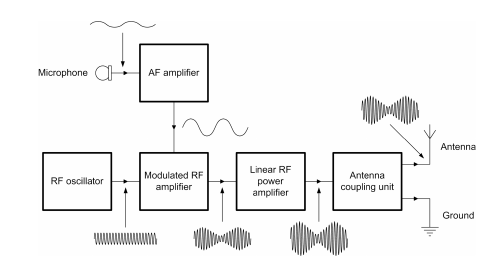
\includegraphics[width=0.75\textwidth]{09.sintesis.comunicaciones.a.bordo/Imagenes.U09/transmisor_am_low-level_modulation.png}
  \caption{Transmisor AM con baja modulación, Fuente: \protect\cite{Tooley_Aircraft_communications_and_navigation_systems}.}
  \label{fig:AM_transmision_baja_modulacion}
\end{figure}


\begin{figure}[!htb]
  \centering
  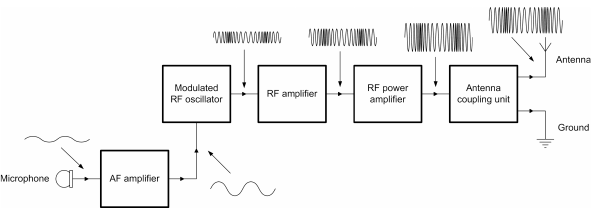
\includegraphics[width=0.75\textwidth]{09.sintesis.comunicaciones.a.bordo/Imagenes.U09/transmisor_fm.png}
  \caption{Transmisor FM, Fuente: \protect\cite{Tooley_Aircraft_communications_and_navigation_systems}.}
  \label{fig:FM_transmision}
\end{figure}


\subsection{Receptor}
\label{sec:09.01.03.receptor}



\begin{figure}[!h]
  \centering
  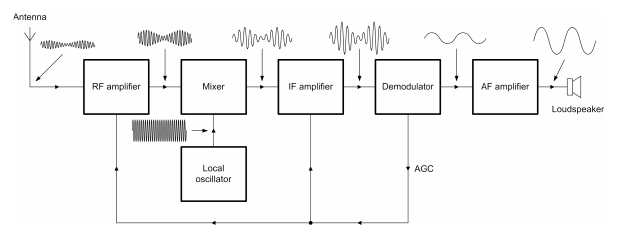
\includegraphics[width=0.75\textwidth]{09.sintesis.comunicaciones.a.bordo/Imagenes.U09/receptor_superheterodino.png}
  \caption{Receptor superheterodino: \protect\cite{Tooley_Aircraft_communications_and_navigation_systems}.}
  \label{fig:receptor.superheterodino}
\end{figure}

\subsection{Equipos integrados}
\label{sec:09.01.04.equipos.integrados}

Usualmente los equipos de comunicaci\'on por radio integran en uno solo a al transmisor y al receptor, lo cual se suele denominar transceptor.

Al principio se empleaban bandas de frecuencias  LF y MF debido a que los equipos disponibles no pod\'ian operar en mayores frecuencias. Luego aparecieron los equipos HF con rango de frecuencias entre 2 y 30 MHz, potencias entre 80 a 200 W, y antenas largas emple\'andose usualmente cables que un\'ian el estabilizador vertical con la parte delantera del fuselaje. Como permit\'ian mantener comunicaciones de hasta 2000 millas n\'auticas se emplearon en aeronaves que recorrieran grandes distancias.

Actualmente las aeronaves de corto alcance emplean el rango de VHF o UHF, aunque con el inconveniente de que su alcance es reducido debido al tipo de onda de radio, ver p\'agina \pageref{sec:A.07.propagacion.ondas.radio}. Con VHF se alcanzan distancias m\'aximas de 250 nm y frecuencias de emisi\'on entre 118 y 137 MHz, con potencias entre 5 y 25 W.


% \subsubsection{Transceptor de VHF}
% \label{sec:09.01.04.01.transceptor.VHF}

% En la Figura xxx se presenta un diagrama de bloques de un equipo VHF de uso aeron\'autico, en el mismo se observan:

% \begin{itemize}
% \item {\bf Circuitos de interfase}
% \item {\bf Circuitos de control}
% \item {\bf Sintetizador de frecuencia}
% \item {\bf Receptor}
% \item {\bf Circuitos atenuadores de ruido (squelch)}
% \item {\bf Circuito de audio del receptor}
% \item {\bf Transmisor}
% \item {\bf Circuito modulador}
% \item {\bf Circuitos de la fuente de alimentaci\'on:} consisten en un filtro LC, un circuito protector contra sobrevoltajes, dos reguladores de CC de $\pm 12$ V de CC, un regulador de $\pm 5$ V de CC y un regulador de interrupci\'on de $\pm 16$ V de CC.  Con estos circuitos se proporciona la energ\'ia el\'ectrica para alimentar a los sistemas del transceptor excepto al circuito integrado del sintetizador y el amplificador de sintonizaci\'on de tensi\'on, los cuales poseen reguladores por separado de $\pm 5$ V de CC y $\pm 23$ V de CC.
% \end{itemize}


% \subsubsection{Transceptor de UHF}
% \label{sec:09.01.04.02.transceptor.UHF}





\subsection{Otros sistemas de comunicaciones}
\label{sec:09.01.05.otros.sistemas.comunicaciones}

En estos \'ultimos tiempos han aparecido nuevos sistemas de comunicaciones, entre ellos se tienen a las comunicaciones por sat\'elite (SATCOM), los sistemas SELCAL, etc.

\section{Otros equipos del sistema de radio}
\label{sec:09.02.otros.equipos.del.sistema.de.radio}

Se emplean otros equipos adicionales como ser auriculares y micr\'ofono para facilitar la comunicaci\'on entre la tripulaci\'on y el equipo de tierra, ya sea en control de tr\'ansito como mec\'anicos.

Otros equipos necesarios son cajas de control de radio, antenas, cajas de audio, amplificador. \'Este \'ultimo se emplea para aumentar la potencia de transmisi\'on.

\subsection{Caja de control}
\label{sec:09.02.01.caja.de.control}

Permite seleccionar diversas funciones del equipo, han evolucionado desde los controles manuales a los digitales que mediante software permiten al usuario  modificar a su gusto diversas operaciones, permitiendo seleccionar canales, frecuencias fijas de emisi\'on, comunicaciones en ``Have Quick'' (HQ), enlaces tipo ``Data Link'' (DL), comunicaciones seguras ``Secure Voice'' (SV), etc.

\subsection{Antena}
\label{sec:09.02.02.antena}

Se emplea usualmente la denominada Marconi o de lambda cuartos. Su longitud es un poco m\'as corta que la cuarta parte de la longitud de onda. 

\begin{table}[!h]
  \centering
  \caption{Dimensiones antena lambda cuartos, adptado de \protect\cite{martnez2006sistemas}}
  \label{tab:09.dimensiones.antena.lambda.cuartos}

  \begin{tabular}{cccc} \hline \rowcolor{cyan!20}
{\bf Radio} & {\bf Frecuencia [MHz]} & {\bf Longitud onda [m]} & {\bf Longitud antena [cm]} \\ \hline
HF & 2 & 150 & 3750 \\ 
& 30 & 10 & 250 \\ \hline
VHF & 118 & 2,5 & 63 \\ 
& 152 & 2 & 5 \\ \hline
UHF & 231 & 1,3 & 32 \\
& 399 & 0,75 & 19 \\ \hline
    
  \end{tabular}
\end{table}

\begin{figure}[!htb]
  \centering
  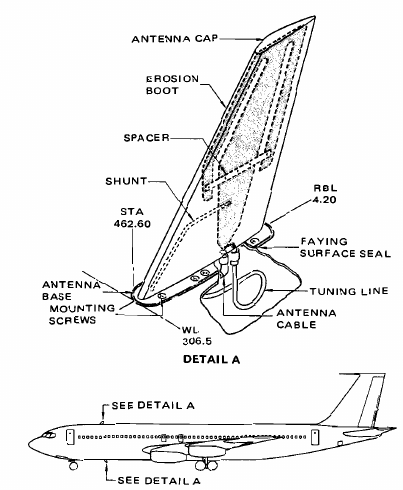
\includegraphics[width=0.5\textwidth]{09.sintesis.comunicaciones.a.bordo/Imagenes.U09/antena_vhf.png}
  \caption{Antena de VHF en una aeronave, Fuente: \protect\cite{eismin1994aircraft}.}
  \label{fig:vhf.antena.aeronave}
\end{figure}


\begin{figure}[!htb]
  \centering
  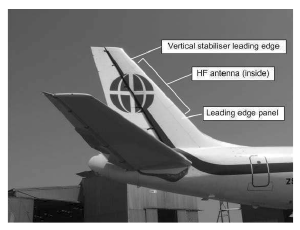
\includegraphics[width=0.5\textwidth]{09.sintesis.comunicaciones.a.bordo/Imagenes.U09/antena_hf.png}
  \caption{Antena de HF en una aeronave, Fuente: \protect\cite{Tooley_Aircraft_communications_and_navigation_systems}.}
  \label{fig:vhf.antena.aeronave}
\end{figure}


Para los casos de la Tabla \ref{tab:09.dimensiones.antena.lambda.cuartos} se observa que para cada tipo de se\~nal se tiene un rango de longitudes de antena, por lo cual se termina  eligi\'endose una longitud intermedia para poder barrer todo el margen de frecuencias sin mayores p\'erdidas. 



\subsection{Caja de audio}
\label{sec:09.02.03.caja.audio}

Es un equipo electr\'onico embarcado cuya misi\'on es controlar el volumen de sonido proporcionado a los tripulantes de los distintos sistemas de navegaci\'on y comunicaciones. Se encuentra integrado por una serie de circuitos amplificadores transistorizados que tratan las se\~nales recibidas de los diferentes sistemas. La operaci\'on se realiza por medio de dos canales conmutables de amplificaci\'on normal y de emergencia.

En el frente del equipo se tienen varios botones pulsadores asociados con algunos potenci\'ometros, los cuales controlan de forma constante el volumen de audio de los receptores y del sistema de intercomunicaci\'on de a bordo. 
De la misma forma se controla la modulaci\'on de los transmisores asociados a los receptores y al intercomunicador de a bordo.

Es posible utilizar varios canales de transmisi\'on simultaneamente.

Los dos sistemas, intercomunicadores e interfonos, se controlan con la caja de audio, que permite subir o bajar el volumen seg\'un las condiciones sonoras existentes.

\section{Sistemas avanzados}
\label{sec:09.03.sistemas.avanzados}

\subsection{Sistema CAMU}
\label{sec:09.03.01.CAMU}

La Unidad de Gesti\'on de Comunicaciones y Audio, en ingl\'es \ac{CAMU}, consiste en una computadora que controla las comunicaciones de la aeronave.

Como coraz\'on de las comunicaciones gestiona el camino de comandos de audio, enlaces entre cabina y los diferentes componentes del sistema, produce los mensajes de voz y los ``{\it warnings}'', y proporciona alternativas a los fallos de los componentes del sistema. Una de sus funciones principales consiste en acondicionar las se\~nales de audio, mezclar, comparar y amplificar con patrones. Se emplean tres t\'ecnicas para el acondicionamiento:

\begin{itemize}
\item {\bf \ac{NAM}}, asegura la inteligibilidad del audio y minimiza la fatiga auditiva de los tripulantes.
\item {\bf \ac{VOGAD}}, mantiene la se\~nal del micr\'ofono de forma autom\'atica y continua sobre el nivel de ruido.
\item {\bf \ac{VOS}}, asegura el cierre de la l\'inea del micro cuando \'este no est\'a en uso.
\end{itemize}

El equipo est\'a compuesto por varios m\'odulos:

\begin{itemize}
\item Un procesador
\item Dos m\'odulos de comunicaciones y audio
\item Dos m\'odulos generadores de audio de alerta
\item Un m\'odulo de conmutaci\'on y filtrado de audio
\item Un m\'odulo de reconocimiento de voz
\item Un m\'odulo terminal para el bus de datos externo
\end{itemize}

El sistema de comunicaciones se compone de dos radios, una de ellas junto con el CAMU son alimentadas por CC de bater\'ias, para poder establecer comunicaciones antes de conectar la APU o GPU. 

\subsection{Sistema DVI}
\label{sec:09.03.02.DVI}

El Sistema de Entrada Directa por Voz, en ingl\'es  \ac{DVI},  permite al piloto manejar con un procedimiento
alternativo la cabina y los sistema de la aeronave.  El sistema forma parte del \ac{CAMU} como un subconjunto funcional interior.

El sistema consiste en un m\'odulo reconocedor de sonidos que enlaza algunos buses de datos con los controles y pantallas de cabina. Su principio se basa en el reconocimiento de sonidos en lugar de palabras, para mejorar la identificaci\'on y comprensi\'on de la pronunciaci\'on de cada persona en particular, el sistema permite cargar unas plantillas personalizadas que se pueden descargar en la aeronave por medio del M\'odulo Portable de Datos, en ingl\'es \ac{PDS}. 

No es empleado en controles que impliquen funciones que afecten a la seguridad, por ejemplo bajar el tren de aterrizaje.

Para habilitar el sistema el piloto presiona un control y da la orden verbal al sistema terminando con una orden ejecutiva, usualmente un GO!. Al dejar de presionar el control el sistema deja de recibir la informaci\'on. 

El sistema presenta en pantalla la orden dada por el piloto y genera una se\~nal audible para que lo escuche el piloto. Al detectar la orden ejecutiva se muestra su ejecuci\'on parpadeando unos segundos en pantalla.

El vocabulario empleado se limita a una centena de palabras.

El DVI es capaz de responder por voz a la pregunta que haya efectuado el piloto.

\subsection{Sistema MIDS}
\label{sec:09.03.03.MIDS}

El Sistema Multifunci\'on de Distribuci\'on de Informaci\'on, en ingl\'es \ac{MIDS}, es un sistema de tipo digital de gran capacidad con flexibilidad y seguridad en el intercambio de informaci\'on en tiempo real.

Se utiliza en aeronaves de combate y proporciona el enlace de datos a la red de información estandarizada Link 16 de la OTAN. Cada integrante de la red posee un n\'umero de identificaci\'on que permite diferenciarlo del resto, y puede intercambiar informaci\'on con los dem\'as respecto a su posici\'on, estado, amenazas, zonas seguras, etc. Tambi\'en se permite ordenar movimientos dentro del escenario de combate y asignar misiones a sus integrantes.

El sistema de transmisión de datos digital MIDS (Multifunctional Information Distribution System)  que sirve para intercambiar informaciones tácticas (como por ejemplo trayectorias de vuelo, objetivos, posición, estatus y órdenes) entre diferentes unidades o plataformas militares en misiones conjuntas o combinadas.

\href{http://tda-armements.com/sites/default/files/asset/document/13-mids_lvt_euromids_2010_bis_0.pdf}{Folleto de MIDS}

\href{https://www.viasat.com/products/link-16-mids-lvt1}{Viasat MIDS Link 16 }

\href{https://en.wikipedia.org/wiki/Link_16}{Link 16}

Est\'a conformado por los siguientes equipos:

\begin{itemize}
     \item MIDS LVT, en ingl\'es \ac{LVT}, interfaz de la red.
     \item MIDS MIU, en ingl\'es \ac{MIU},recibe los mensajes y genera los datos de comando. Gestiona las transmisiones LVT a la red, enviando los datos del MIDS al sistema de avi\'onica y de cabina.
     \item Antena interior en banda D
     \item Antena combinada en la deriva
\end{itemize}

Las funciones del MIDS son:

\begin{itemize}
\item Participaci\'on en la red
\item Gestión de trayectorias e intercambio de la informaci\'on t\'actica
\item Gesti\'on de mando y control
\item Suministro de m\'etodos de transmisi\'on segura de la voz
\item Definici\'on y env\'io de mensajes alfanum\'ericos de texto
\item Gesti\'on de funciones \ac{A/A} y \ac{A/S} del \ac{TACAN}
\end{itemize}





% \section{Comunicaciones en VHF}
% \label{sec:09.comunicaciones.VHF}


% \cite{kayton_avionics_navigation_systems}

% La radio de Muy Alta Frecuencia, en ingl\'es \ac{VHF}, ha sido durante mucho tiempo el principal medio de comunicación entre una aeronave y la base en tierra. El sistema funciona en el rango de frecuencia que se extiende desde 118 MHz a 137 MHz y admite la comunicación de voz y datos (esta última cada vez más importante). 
%  La comunicación \ac{VHF} se utiliza para diversos fines, incluido el \ac{ATC}, la información de aproximación y salida, la transmisión de información meteorológica, el manejo en tierra de las aeronaves, las comunicaciones de la empresa aérea y también para el Sistema de Comunicaciones e Informes de Aeronaves, en ingl\'es  \ac{ACARS}.


% \subsection{Rango de VHF y propagación}
% \label{sec:09.01.rango.VHF}

% En el rango de VHF (30 MHz a 300 MHz), las ondas de radio generalmente se propagan como Línea de Visión Directa
% (LOS), ver p\'agina \pageref{sec:A.07.propagacion.ondas.radio}. La propagación de la onda de cielo todavía ocurre en el extremo inferior del rango de VHF (hasta aproximadamente 50 MHz dependiendo de la actividad solar) pero en las frecuencias utilizadas para la comunicación de la aeronave, la reflexión desde la ionosfera es excepcionalmente rara. La comunicación por rutas de LOS, aumentada en ocasiones por difracción y reflexión, impone un límite en el rango de trabajo. eso se puede obtener. También debería ser evidente que el alcance dependerá de la altura de una aeronave sobre el suelo; cuanto mayor sea, mayor será el rango. La distancia máxima de LOS (ver Figura 4. 1) entre un avión y una estación terrestre en millas náuticas (nm), viene dada por la relación:

% donde está la altitud del avión en pies sobre el suelo (se supone que es un terreno plano).

% Ejemplo 4.1

% Determine la distancia máxima de la línea de visión cuando una aeronave vuela a una altura de (a) 2500 pies y (b) 25000 pies.

% El alcance real obtenido depende no solo de la distancia LOS sino también de varios otros factores, incluida la posición de la aeronave, la potencia del transmisor y la sensibilidad del receptor. Sin embargo, la distancia LOS generalmente proporciona una buena aproximación del alcance que se puede obtener entre un avión y una estación terrestre (ver Tabla 4. 1). La situación es un poco más compleja cuando la comunicación es de un avión a otro; sin embargo, en tales casos, sumar las dos distancias LOS normalmente proporcionará una guía sobre el rango máximo que se puede esperar.

% Pon a prueba tu comprensión 4.1

% Determine la altitud de un avión que proporcionaría una distancia de línea de visión a una estación terrestre ubicada a una distancia de 125 nm.

% \subsection{Modulación DSB}
% \label{sec:09.02.modulacion.DSB}


% Modulación de amplitud 1s utilizada para comunicaciones de voz, así como varios de los modos de enlace de datos VHF (VDL). El sistema utiliza la modulación de doble banda lateral (DSB) y, dado que esto tiene implicaciones para el ancho de banda de las señales moduladas, vale la pena dedicar un poco de tiempo a explicar cómo funciona esto antes de ver cómo se divide el espacio disponible en canales. La Figura 4.2 muestra el espectro de frecuencia de una onda portadora de RF a 1 24.575 MHz de amplitud modulada por un solo tono sinusoidal puro con una frecuencia de 1 kHz. Observe cómo la forma de onda modulada en amplitud comprende tres componentes separados:

% un portador de RF a 1 24.575 MHz

% un componente de frecuencia lateral inferior (LSF) a 1 24.574 MHz

% un componente de frecuencia del lado superior (USF) a 1 24.576 MHz.


% Observe cómo el LSF y el USF están separados de la portadora de RF por una frecuencia que es igual a la de la señal de modulación (en este caso, 1 kHz). Observe también en la Figura 4.2 que el ancho de banda (es decir, el rango de frecuencias ocupadas por la señal modulada) es el doble de la frecuencia de la señal moduladora (es decir, 2 kHz).

% La figura 4.3 muestra una portadora de RF modulada por una señal de voz en lugar de un solo tono sinusoidal. La señal de banda base (es decir, la señal de voz en sí) generalmente ocupa un rango de frecuencia que se extiende desde alrededor de 300 Hz a 3 .4 kHz. De hecho, para mejorar la inteligibilidad y reducir el ruido extraño, la respuesta de frecuencia del micrófono y el amplificador de voz está invariablemente diseñada para seleccionar este rango particular de frecuencias y rechazar cualquier señal de audio que se encuentre fuera de él. De la Figura 4.3 se debe tener en cuenta que el ancho de banda de la señal de RF es de aproximadamente 7 kHz (es decir, el doble que la señal de modulación más alta).

% Pon a prueba tu comprensión 4.2

% Determine los componentes de frecuencia de la señal de RF presentes en una onda portadora modulada en amplitud DSB a 1 1 8.975 MHz cuando la señal de modulación comprende tonos puros a 2 kHz y 5 kHz.

% \subsection{Espaciado de canales}
% \label{sec:09.03.espaciado.canales}

% Las comunicaciones de la aeronave VHF se realizan en varios canales ubicados. Estos canales estaban originalmente espaciados a intervalos de 200 kHz en toda la banda de aviones VHF. Sin embargo, un aumento incesante en el tráfico aéreo, junto con el uso cada vez mayor de sistemas de aviónica para la comunicación de enlace de datos, ha puesto una demanda creciente en el espectro de frecuencia disponible. En respuesta a esta demanda, la separación entre canales adyacentes en la banda 1 1 8 MHz a 1 3 7 MHz se ha reducido sucesivamente para aumentar el número de canales disponibles para la comunicación VHF (ver Tabla 4.2).

% La Figura 4.4 muestra el espaciado de canales para los sistemas VHF europeos anteriores de 25 kHz y actuales de 8.33 kHz. Observe cómo el sistema de espaciado de canales de 8.33 kHz permite que tres señales DSB AM ocupen el espacio que anteriormente estaba ocupado por
% Una sola señal.

% La desventaja del espaciado de canales estrechos es que la banda de protección del espectro no utilizado que existía anteriormente con el sistema de 25 kHz está completamente ausente y que los receptores deben diseñarse de modo que tengan un grado muy alto de rechazo de canal adjunto (consulte la página 48) . También se deben tomar medidas para garantizar que el ancho de banda de la señal transmitida no exceda los 7 kHz, o sea, el ancho de banda requerido para una comunicación de voz efectiva. La penalidad por no restringir el ancho de banda es que las señales de un canal pueden 'extenderse' a los canales adyacentes, causando interferencia y degradando la comunicación (ver Figura 4.7).

% Tabla: aumento en la cantidad de canales VHF disponibles

% Pon a prueba tu comprensión 4.3

% ¿Cuántos canales con una separación de 1 2. 5 kHz pueden ocupar la banda que se extiende desde 1 1 8 MHz a 1 25 MHz?

% Pon a prueba tu comprensión 4.4

% Un total de 1 520 canales de datos se acomodarán en una banda que se extiende desde 3 1 6 MHz hasta 335 MHz. ¿Qué espacio de canal debe usarse y qué rango de frecuencias puede tener la señal de banda base?


% \subsection{Profundidad de modulación}
% \label{sec:09.04.profundidad.modulacion}

% La profundidad de modulación de una onda portadora de RF generalmente se expresa en términos de modulación porcentual, como se muestra en la Figura 4.6. Tenga en cuenta que el nivel de modulación puede variar entre 0\% (correspondiente a una portadora completamente no modulada) a 100\% (correspondiente a una portadora completamente modulada).

% En la práctica, la inteligibilidad de una señal (es decir, la capacidad de recuperar información de una señal débil que puede verse afectada negativamente por el ruido y otras perturbaciones) aumenta a medida que aumenta la modulación porcentual y, por lo tanto, es necesario garantizar que la señal está completamente modulada pero sin el riesgo de sobremodulación (ver Fig. 4.6). El resultado de la sobremodulación es un ancho de banda excesivo, o 'salpicadura', que causa interferencia del canal adjunto, como se muestra en la figura 4.7.

% \subsection{Compresión}
% \label{sec:09.05.compresion}

% Para mejorar la inteligibilidad de las comunicaciones de voz VHF, la etapa de amplificador de voz de una radio VHF de avión está invariablemente equipada con una etapa de compresor. Esta etapa proporciona alta ganancia para señales de baja amplitud y ganancia reducida para señales de alta amplitud. El resultado es un aumento en la profundidad de modulación promedio (ver Figura 4.8).

% La figura 4.9 muestra las características típicas del amplificador de voz con y sin compresión. Tenga en cuenta que la mayoría de los equipos de radio VHF de la aeronave proporcionan ajustes tanto para el nivel de modulación como para la cantidad de compresión que se aplica (ver Figura 4. 1 0).

% Portadora de RF modulada que muestra diferentes cantidades de compresión aplicadas a la señal de modulación

% \subsection{Silenciamiento}
% \label{sec:09.06.silenciamiento}

% Los receptores VHF de aviones incorporan invariablemente un sistema de silenciar las etapas de audio del receptor en ausencia de una señal entrante. Este sistema está diseñado para eliminar el molesto y molesto ruido de fondo que está presente cuando no se reciben señales. Dichos sistemas se denominan silenciador y el umbral en el que funciona se ajusta (consulte la Figura 4. 1 0) para que el silenciador 'se abra' para una señal débil pero se 'cierre' cuando no hay señal presente.

% Se utilizan dos sistemas de silenciador bastante diferentes, pero el sistema más común (y fácil de implementar) responde a la amplitud de la portadora recibida y se conoce como silenciador operado por la portadora. El voltaje utilizado para inhibir el audio del receptor puede derivarse del sistema AGC del receptor y alimentarse a la puerta de silenciamiento (Figura 4. 1 1).


% El sistema de silenciador alternativo (y algo superior) implica detectar el ruido presente en la salida de la etapa del detector del receptor y usarlo para desarrollar una señal de control que depende de la relación señal / ruido de la señal recibida en lugar de su amplitud. Esta última técnica, que no solo ofrece una mejor sensibilidad, sino que también es menos propensa a dispararse por el ruido de fondo general y las señales fuera del canal, a menudo se encuentra en los receptores de FM y se conoce como silenciador operado por ruido.

% \subsection{Modos de datos}
% \label{sec:09.07.modos.de.datos}

% Los modernos equipos de comunicaciones VHF de aviones admiten tanto la comunicación de datos como la comunicación de voz. El sistema utilizado para la tinta de datos de la aeronave se conoce como Sistema de direccionamiento e informe de comunicaciones de aeronaves (ACARS). Actualmente, los aviones están equipados con tres radios VHF, dos de los cuales se usan para comunicaciones de voz A TC y uno se usa para el enlace de datos ACARS (también conocido como comunicaciones de control operativo de la aerolínea).

% Un terminal de enlace de datos a bordo del avión (ver Figura 4. 1 2) genera mensajes de enlace descendente y procesa los mensajes de enlace ascendente recibidos a través del enlace de datos VHF. Los mensajes ACARS de enlace descendente y enlace ascendente están codificados como texto ASCII sin formato. En los Estados Unidos, las estaciones terrestres ACARS son operadas por ARINC, mientras que en Europa, Asia y América Latina, el servicio equivalente es proporcionado por SIT A.

% Inicialmente, a cada proveedor ACH VHF se le asignó un solo canal VHF. Sin embargo, a medida que ha crecido el uso de enlaces de datos VHF (VDL), el número de canales utilizados en las cercanías de los aeropuertos más activos ha aumentado hasta cuatro y estos a menudo funcionan a plena capacidad.

% Desafortunadamente, debido a la presión por canales de voz adicionales, no ha sido posible asignar un número de canales VHF adicionales para la operación del enlace de datos ACARS. Como resultado, recientemente se han introducido varios modos de datos nuevos que admiten velocidades de datos más altas y hacen un uso más eficiente de cada canal de 25 kHz actualmente asignado para fines de enlace de datos.

% Además, la FAA está desarrollando un sistema que permitirá la integración de comunicaciones de voz y datos ATC. Este sistema utiliza audio codificado digitalmente en lugar de señales de voz analógicas convencionales.

% Cuando se opera en modo VDL 0, los protocolos de enlace de datos requeridos se implementan en la unidad de administración A CARS (consulte la Figura 4. 1 1).

% Los datos se transfieren desde la radio VHF a la unidad de gestión a una velocidad de 2400 bits por segundo (bps) mediante la codificación por desplazamiento de frecuencia (FSK).

% La señal de audio FSK consta de dos tonos sinusoidales, uno a 1 .2 kHz y otro a 2 .4 kHz, dependiendo de si la polaridad del bit de información que se transmite es la misma que la del bit anterior o es diferente. Tenga en cuenta que la fase de los tonos varía linealmente y que no hay cambio de fase en la transición entre los dos tonos.

% Este tipo de modulación (en la que el espaciado de frecuencia entre los dos tonos de audio es exactamente la mitad de la velocidad de datos) es altamente eficiente en términos de ancho de banda y, por lo tanto, se conoce como desplazamiento mínimo (MSK). Cuando se transmiten los datos, la señal MSK se usa para modular la amplitud de la portadora VHF (en gran parte igual que la señal de voz). La señal transmitida resultante es entonces una señal AM de doble banda lateral (DSB) cuya amplitud se modula a 2400 bps. Luego se dice que el portador de RF usa la modulación DSB AM MSK.

% La selección de frecuencia de portadora VHF y el control de transmisión / recepción son proporcionados por la unidad de gestión ACARS que trabaja en conjunción con una interfaz ARINC 429 a la radio VHF (Figura .1. 1 2). El protocolo de acceso al canal empleado se define como CSMA de acceso múltiple con detección de portadora). Consiste en escuchar la actividad en el canal (es decir, transmisiones de otros usuarios) 3. La transmisión solo se realiza cuando el canal está libre.

% La operación en el Modo VDL A es similar al Modo 0, excepto que los paquetes de datos ACARS de enlace ascendente y descendente se transfieren entre la radio VHF y la unidad de gestión ACARS a través de un par de transmisión / recepción de interfaces digitales ARINC 429 de 1 00 kbps en lugar de la interfaz de audio analógica utilizada por Modo 0. Los datos digitales son utilizados por la radio VHF para modular la portadora de RF a una velocidad de 2400 bps usando el mismo esquema de modulación DSB AM MSK utilizado por el Modo 0 de VDL.

% Otra diferencia entre el Modo VDL 0 y el Modo VDL A es que, cuando se usa este último, la radio VHF controla cuándo acceder al canal para transmitir datos usando el mismo protocolo CSMA empleado por la unidad de gestión en el Modo VDL 0. Sin embargo, la selección de la frecuencia que se utilizará todavía está controlada por la CMU o ATSU mediante comandos emitidos a través de la misma interfaz ARINC .f29 utilizada para la transferencia de datos. Tenga en cuenta que, en lo que respecta a las estaciones terrestres de enlace de datos VHF, no hay diferencia en las transmisiones VDL Modo 0 aire / tierra VDL Modo A.

% La operación en Modo VDL 2 se basa en un conjunto mejorado de protocolos de transferencia de datos y, como resultado, proporciona un aumento significativo en la capacidad de datos. VDL Mode 2 ha sido diseñado para proporcionar la migración futura de VDL a la Red de Telecomunicaciones Aeronáuticas, en ingl\'es \ac{ATN}.

% Esta red permitirá una entrega más eficiente y sin problemas de mensajes de datos y archivos de datos entre aeronaves y los sistemas informáticos terrestres utilizados por las aerolíneas y las instalaciones de control de tráfico aéreo.

% \ac{ATN} será apoyado por una serie de redes aéreas / terrestres y redes terrestres / terrestres.

% Las redes aire / tierra y tierra / tierra estarán interconectadas por medio de enrutadores A TN que implementan los protocolos requeridos y funcionarán de la misma manera que Internet con la que probablemente ya esté familiarizado.

% El Modo VDL 2 emplea una velocidad de datos de 31500 bits por segundo a través del enlace aire / tierra usando un solo canal de 25 kHz. La mayor utilización del canal de 25 kHz se logra empleando un sistema de modulación que es más eficiente en términos de uso de ancho de banda. Este sistema se conoce como modulación por desplazamiento de ocho fases diferencial (D8PSK). En este sistema, una señal portadora de audio se modula mediante un cambio de fase que puede tomar una de las ocho fases posibles; 0º, 45º, 90º, 135º, 180º, 225º, 270º o 315º. Estos cambios de fase corresponden a tres bits de datos digitales de la siguiente manera: 000, 001, 011, 010, 110, 111, 101 o 100. El modulador D8PSK utiliza los bits en mensaje de datos, en grupos de tres, para determinar el cambio de fase de la portadora a una velocidad de 10,5 kHz.

% En consecuencia, la velocidad de bits será tres veces este valor, o 31.5 kBps. La modulación D8PSK de la fase de la portadora VHF se logra utilizando un modulador de cuadratura. Tenga en cuenta que, en la modulación D8PSK, los grupos de tres bits a menudo se denominan símbolos D8PSK.

% VDL Mode 3 ofrece una alternativa a la solución europea de reducir el espacio entre canales a 8.33 kHz. El Modo VDL 3 toma una asignación de frecuencia de 25 kHz y la divide en 1 tramas de 20 ms con cuatro intervalos de tiempo de 30 ms (cada uno de los cuales constituye un canal diferente). Por lo tanto, el Modo 3 emplea la multiplexación por división de tiempo (TDM) en lugar de la multiplexación por división de frecuencia (FDM) utilizada en el sistema europeo. Tenga en cuenta que el Modo VDL 3 es el único modo VDL planificado que está diseñado para admitir el tráfico de voz y datos en la misma frecuencia.


% \subsection{ACARS}
% \label{sec:09.08.ACARS}

% El \ac{ACARS} es un sistema de enlace de datos digitales transmitido en el rango VHF (118 MHz a 136 MHz). \ac{ACARS} proporciona un medio por el cual los operadores de aeronaves pueden intercambiar datos con una aeronave sin intervención humana. Esto hace posible que una aerolínea se comunique con la aeronave de su flota de la misma manera que es posible intercambiar datos utilizando una red digital terrestre. \ac{ACARS} utiliza el identificador único de una aeronave y el sistema tiene algunas características que son similares a las utilizadas actualmente para el correo electrónico.

% El sistema \ac{ACARS} se especificó originalmente en el estándar ARINC 597, pero se ha revisado como ARINC 724B. Una característica importante de \ac{ACARS} es la capacidad de proporcionar datos en tiempo real sobre el terreno relacionados con el rendimiento de la aeronave; Esto ha permitido identificar y planificar actividades de mantenimiento de aeronaves.

% Las comunicaciones ACARS se dirigen automáticamente a través de una serie de computadoras \ac{ARINC} con base en tierra al operador de la aeronave correspondiente. El sistema ayuda a reducir la necesidad de mensajes de voz mundanos en HF y VHF y proporciona un sistema que puede registrarse y rastrearse. Los mensajes ACARS típicos se usan para transmitir información de rutina como:

% \begin{itemize}
%      \item cargas de pasajeros
%      \item informes de salida
%      \item informes de llegada
%      \item datos de combustible
%      \item datos de rendimiento del motor.
% \end{itemize}

% Esta información puede ser solicitada por la compañía y recuperada de la aeronave a intervalos periódicos o bajo demanda. Antes de ACARS, este tipo de información se habría transferido a través de voz VHF. ACARS utiliza una variedad de componentes de hardware y software, incluidos los que están instalados en el suelo y los que están presentes en la aeronave. Los componentes ACARS de la aeronave incluyen una unidad de gestión (ver Figura 4. 1 2) que se ocupa de la recepción y transmisión de mensajes a través del transceptor de radio VHF, y la unidad de control que proporciona la interfaz de la tripulación y consta de una pantalla de visualización e impresora. La red terrestre ACARS comprende las estaciones remotas de transmisión / recepción ARARC ACARS y una red de computadoras y sistemas de conmutación. El subsistema de comando, control y gestión de ACARS consiste en las operaciones de la aerolínea con base en tierra y las funciones asociadas, incluido el control de operaciones, el mantenimiento y la programación de la tripulación.

% Hay dos tipos de mensajes ACARS; mensajes de enlace descendente que se originan en la aeronave y mensajes de enlace ascendente que se originan en estaciones terrestres (véanse las Figuras 4. 1 4 a 4. 1 7). Las frecuencias utilizadas para la transmisión y recepción de mensajes ACARS están en la banda que se extiende desde 1 29 MHz a 1 3 7 MHz (VHF) como se muestra en la Tabla 4.4. Tenga en cuenta que se utilizan diferentes canales en diferentes partes del mundo. Un mensaje ACARS típico (ver Figura 4. 1 4) consiste en:

% \begin{itemize}
%      \item Identificador de modo (por ejemplo, 2)
%      \item Identificador de la aeronave (por ejemplo, G-DBCC)
%      \item Etiqueta de mensaje (por ejemplo, solicitud de clima SU-a)
%      \item Identificador de bloque (por ejemplo, 4)
%      \item Número de mensaje (por ejemplo, M55A)
%      \item Número de vuelo (por ejemplo, BD0 1NZ)
%      \item Contenido del mensaje (ver Figura 4. 1 4).
% \end{itemize}



% Pon a prueba tu comprensión 4.5

% Explique la necesidad de (a) compresión del habla y (b) silenciamiento en la radio VHF de un avión.

% Pon a prueba tu comprensión 4.6

% Explique, con la ayuda de un diagrama de bloques, cómo es posible la transferencia de datos utilizando una radio VHF de avión.

% Pon a prueba tu comprensión 4.7


% Explique la diferencia entre la modulación MSK y DBPSK. ¿Por qué es este último superior?

% \subsection{Equipo de radio VHF}
% \label{sec:09.09.equipo.VHF}

% La especificación típica de una radio de datos VHF de un avión moderno se muestra en la Tabla 4. 5) Esta radio se puede utilizar con voz analógica y datos en los modos 0, A y 2 (consulte la página 65). Las Figuras 4. 1 8 a 4.20 muestran el equipo típico y las ubicaciones de control en un avión de pasajeros, mientras que las Figuras 4.2 1 a 4.24 muestran las vistas internas y externas de una radio VHF típica. Finalmente, la Figura 4.25 muestra una antena de hoja de cuarto de onda VHF típica instalada en un avión Airbus A380.





% \section{Comunicaciones en UHF}
% \label{sec:09.comunicaciones.UHF}

% La radio de alta frecuencia (HF) proporciona  medios de comunicación efectivos a las aeronaves, a través de rutas oceánicas y transpolares de larga distancia. Además, la comunicación de datos global se ha hecho posible recientemente utilizando estaciones terrestres de enlace de datos HF (HFDL) estratégicamente ubicadas. Estos proporcionan acceso a las redes de líneas aéreas ARINC y SITA. Por lo tanto, la comunicación en ondas decamétricas ya no está restringida a la oficina y está experimentando un resurgimiento de interés debido a la necesidad de encontrar un medio de comunicación de datos a larga distancia que aumente los enlaces de datos VHF y SATCOM existentes.

% Un sistema de radio HF de aeronave opera en frecuencias puntuales dentro del espectro de HF. A diferencia de la radio VHF de la aeronave, el espectro no se divide en una gran cantidad de canales contiguos, sino que las asignaciones de aeronaves se intercalan con muchos otros servicios, incluidos la transmisión de onda corta, los servicios fijos punto a punto, los servicios marinos y terrestres, u003d servicios de aficionados y aficionados. . Este capítulo describe el equipo utilizado y los diferentes modos en los que funciona.

% 5.1 Rango de HF y propagación

% En el rango de HF (3 MHz a 30 MHz), las ondas de radio se propagan a largas distancias debido a la reflexión de las capas ionizadas en la atmósfera superior.

% Debido a las variaciones en altura e intensidades de las regiones ionizadas, se deben desactivar diferentes frecuencias en diferentes momentos del día y de la noche y para diferentes caminos. También hay alguna variación estacional (particularmente entre invierno y verano). La propagación también puede verse alterada y mejorada durante los períodos de intensa actividad solar.

% El resultado de esto es que la propagación de HF tiene considerables caprichos y es mucho menos predecible que la propagación en VHF.

% Frecuencias elegidas para una ruta de radio particular; e generalmente se establece aproximadamente a mitad de camino entre la frecuencia utilizable más baja (LUF) y la frecuencia máxima utilizable (MUF). El LUF diurno suele estar entre 4 y 6 MHz durante el día, y cae rápidamente después de la puesta del sol a alrededor de 2 MHz. El MUF depende de la temporada y el ciclo de las manchas solares, pero a menudo se encuentra entre 8 MHz y 20 MHz.

% Por lo tanto, una frecuencia típica durante el día para la comunicación de la aeronave podría ser de 8 MHz, mientras que podría ser tan baja como 3 MHz durante la noche. Los rangos típicos están en la región de 500 km a 2500 km y esto efectivamente llena el vacío en la cobertura de VHF (ver Figura 5. 1).

% Como ejemplo de la necesidad de cambiar las frecuencias durante un período de 24 horas, Figura 5. 2 muestra cómo el servicio proporcionado por el servicio oceánico de Santa Maria HF hace uso de diferentes partes del espectro de HF en diferentes momentos del día y de la noche. Observe la correlación entre la tabla de disponibilidad del servicio que se muestra en la Figura 5 .2 (a) y la variación típica en la frecuencia máxima utilizable (MUF) para la ruta de radio entre Madrid y Nueva York.

% Las siguientes bandas de ondas decamétricas están atribuidas al servicio aeronáutico:


% 5.2 modulación SSB

% Desafortunadamente, el espectro disponible para comunicaciones de aeronaves en HF es extremadamente limitado. Como resultado, se toman medidas para restringir el ancho de banda de las señales transmitidas, tanto para voz como para datos.

% La modulación de amplitud de doble banda lateral (DSB) requiere un ancho de banda de al menos 7 kHz, pero esto puede reducirse transmitiendo solo una de las dos bandas laterales. Tenga en cuenta que se puede usar la banda lateral superior (USB) o la banda lateral inferior (LSB) porque ambas contienen la misma información de señal de modulación. Además, es posible reducir (o "suprimir") el operador ya que esto, en sí mismo, no transmite ninguna información.

% Para demodular una señal transmitida sin una portadora, es necesario volver a insertar la portadora en el extremo receptor (esto se hace en la etapa de demodulador donde un oscilador de frecuencia de latido o un oscilador de inserción de portadora reemplaza la señal de portadora faltante en la frecuencia intermedia final -ver Figura 5. 9). La ausencia de la portadora significa que se desperdicia menos energía en el transmisor, que en consecuencia opera con una eficiencia significativamente mayor.

% La figura 5.3 muestra el espectro de frecuencia de una señal de RF utilizando diferentes tipos de modulación de amplitud, con y sin portadora.

% En la figura 5 .3 (a), el modo de transmisión es la modulación de amplitud de doble banda lateral (DSB) convencional con portadora completa. Esta forma de modulación se utiliza para las comunicaciones de aeronaves VHF y se describió anteriormente en el Capítulo 4.

% La figura 5.3 (b) muestra el efecto de suprimir el portador. Este tipo de modulación se conoce como portadora suprimida de doble banda lateral (DSB-SC).

% En los sistemas DSB-SC prácticos, el nivel de la portadora generalmente se reduce en 30 dB o más.
% La señal DSB-SC tiene el mismo ancho de banda general que la señal DSB de portadora completa, pero la reducción en la portadora da como resultado una mayor eficiencia y una menor susceptibilidad a la interferencia heterodina.

% La figura 5.3 (c) muestra el efecto de retirar tanto el portador como la banda lateral superior. La señal resultante se conoce como banda lateral única (SSB), en este caso utilizando solo la banda lateral inferior (LSB). Observe cómo el ancho de banda general se ha reducido a solo alrededor de 3,5 kHz, es decir, la mitad de la señal DSB AM comparable que se muestra en la Figura 5 .3 (a).

% Finalmente, Figura 5. 3 (d) muestra el efecto de retirar el portador y la banda lateral inferior.

% Una vez más, la señal resultante se conoce como banda lateral única (SSB), pero en este caso estamos usando solo la banda lateral superior (USB). Aquí nuevamente, el ancho de banda general se ha reducido a alrededor de 3. 5 kHz. Tenga en cuenta que la comunicación HF de la aeronave requiere el uso de la banda lateral superior (USB). DSB AM también puede estar disponible, pero ahora se usa muy raramente debido al rendimiento superior que ofrece SSB.

% Pon a prueba tu comprensión 5.1

% 1) Explica por qué la radio HF se usa en rutas transoceánicas.

% 2. Explique por qué se utilizan diferentes frecuencias para las comunicaciones de las aeronaves en ondas decamétricas durante el día y por la noche.

% 3. Establezca DOS ventajas de usar S

% 5.3 SELCAL

% Las llamadas selectivas (SELCAL) reducen la carga de la tripulación de vuelo al alertarlos sobre la necesidad de responder a los mensajes entrantes. SELCAL está disponible en HF y VHF pero el sistema se usa más en HF. Esto se debe en parte a la naturaleza intermitente de las comunicaciones de voz en rutas oceánicas largas y en parte al hecho de que los sistemas de silenciamiento son más difíciles de operar cuando se utiliza SSB porque no hay portadora transmitida para indicar que hay una señal presente en el canal.

% El sistema SELCAL de la aeronave se define en el Anexo 10 del Convenio sobre Aviación Civil Internacional (OACI), Volumen 1, 4a edición de 1 985 (enmendado 1 987). El sistema implica la transmisión de una breve ráfaga de tonos de audio.

% Cada código transmitido compone dos pulsos de tono consecutivos, con cada pulso que contiene dos tonos transmitidos simultáneamente.

% Los pulsos tienen una duración de 1 segundo separados por un intervalo de aproximadamente 0.2 segundos. Para garantizar el correcto funcionamiento del decodificador SELCAL, la frecuencia de los tonos transmitidos debe mantenerse con una precisión superior a $\pm$ 0. 1 5\%.

% Los códigos SELCAL se asignan de manera única a aeronaves particulares por el Control de Tráfico Aéreo (ATC).

% Como ejemplo, un código SELCAL transmitido típico podría consistir en una ráfaga de 1 segundo de 312.6 Hz y 977.2 Hz seguido de una pausa de aproximadamente 0. 2 segundos y otra ráfaga de tono de 1 segundo que comprende 346.7 Hz y 977.2 Hz. Tabla 5.1 indica que el código SELCAL transmitido correspondiente es 'AM-BM' y que solo el avión con este código será alertado de la necesidad de responder a un mensaje entrante.

% La señal de RF transmitida por la estación de radio terrestre debe contener (dentro de 3 dB) cantidades iguales de los dos tonos de modulación y la combinación de tonos debe dar como resultado una envolvente de modulación que tenga un porcentaje de modulación nominal lo más alto posible (y en ningún caso menor que 60%).

% Los tonos transmitidos se componen de combinaciones de los tonos enumerados en la Tabla 5. 1)

% Tenga en cuenta que los tonos se han elegido para que no estén relacionados armónicamente (evitando así la posible confusión dentro del decodificador SELCAL cuando los armónicos de las frecuencias de tonos originales pueden estar presentes en la forma de onda demodulada).

% La cobertura global de enlace de datos de alta frecuencia (HFDL) de ARIN C proporciona una capacidad de enlace de datos altamente rentable para los transportistas en rutas oceánicas remotas, así como las rutas polares en latitudes altas donde la cobertura SATCOM no está disponible. HFDL tiene un costo menor que SATCOM y muchos operadores están utilizando HFDL en lugar de servicios satelitales o como un sistema de respaldo. HFDL sigue siendo la única tecnología de enlace de datos que funciona en el Polo Norte, proporcionando una cobertura de enlace de datos continua e ininterrumpida en las rutas polares populares entre América del Norte y Europa del Este y Asia.

% La demanda de HFDL ha crecido de manera constante desde que ARINC lanzó el servicio en 1 998, y hoy todos los principales fabricantes de aviones ofrecen la aviónica HFDL como equipo original. HFDL ofrece una solución rentable para el servicio global de enlace de datos. La demanda del servicio HFDL está creciendo actualmente en más de varios cientos de aviones por año.

% Las ventajas de HFDL se pueden resumir como:

% amplia cobertura debido al rango extremadamente largo de señales de HF

% cobertura simultánea en varias bandas y frecuencias (actualmente 60)

% múltiples estaciones terrestres (actualmente 1 4) en ubicaciones estratégicas de todo el mundo aviónica relativamente simple utilizando tecnología probada

% adquisición rápida de red

% disponibilidad de red excepcional

% Las desventajas de HFDL son:

% velocidades de datos muy bajas (lo que hace que el sistema no sea adecuado para comunicaciones de banda ancha de alta velocidad).

% Como resultado de lo anterior, la gran mayoría de los mensajes HFDL están relacionados con el control operativo de la aerolínea (AOC) (véase la figura 5 .4), pero también se espera que HFDL desempeñe un papel importante en los futuros sistemas de navegación aérea (FANS) donde proporcionará un medio adicional de vinculación de datos con una aeronave, complementando los sistemas VDL, GPS y SATCOM. Tenga en cuenta que SATCOM puede admitir velocidades de datos mucho más rápidas, pero también puede ser susceptible a interrupciones y puede no estar disponible en latitudes altas. HFDL utiliza modulación por desplazamiento de fase (PSK) a velocidades de datos de 300, 600, 1 200 y 1 800 bps. La velocidad utilizada depende de las condiciones de propagación prevalecientes. HFDL se basa en la multiplexación por división de frecuencia (FDM) para acceder a las frecuencias de la estación terrestre y la multiplexación por división de tiempo (TDM) dentro de los canales de comunicación individuales. 5 muestra cómo el espectro de frecuencia de una señal HFDL típica a 300 bps se compara con una señal de voz HF.Figura 5 . 

% La Figura 5.6 muestra mensajes típicos de HFDL enviados desde los cuatro aviones que se muestran en la Figura 5 .7 a la estación terrestre de Shannon HFDL utilizando el mismo canal de comunicaciones. La ruta de radio de uno de los aviones (LH8409) se ilustra en la Figura 5.8. Los primeros dos de los mensajes que se muestran en la Figura 5.6 son solicitudes de inicio de sesión y la velocidad de bits máxima se especifica en el encabezado. En cada solicitud de inicio de sesión, la aeronave se identifica por su dirección única de la OACI de 24 bits. Una vez conectado, el avión recibe un código de dirección de 8 bits (hexadecimal AF en el caso del tercer mensaje y hexadecimal AD en el caso del cuarto mensaje). Cada avión también transmite sus datos de ubicación actuales (longitud y latitud).

% El sistema utilizado para el intercambio de datos HFDL se especifica en ARINC 635. Cada estación terrestre transmite una trama llamada 'squitter' cada 32 segundos. El marco de squitter informa a la aeronave del estado del sistema, proporciona una referencia de sincronización y proporciona control de protocolo. Cada estación terrestre tiene un desplazamiento de tiempo para sus squitters. Esto permite que las aeronaves salten entre estaciones terrestres para encontrar la mejor antes de iniciar sesión. Al pasar el tráfico, se utilizan franjas horarias TDM dedicadas. Esto evita que dos aviones transmitan al mismo tiempo causando cousiones de datos.

% 5.5 equipo de radio HF

% El esquema de bloques de un simple transmisor / receptor de HF se muestra en la Figura 5 .9. Tenga en cuenta que, si bien este equipo usa una sola frecuencia intermedia (IF), en la práctica la mayoría de las radios HF de aviones modernos son mucho más complejas y usan dos o tres frecuencias intermedias.

% En el modo de transmisión, la portadora suprimida DSB (Figura 5 .2b) se produce por medio de una etapa de modulador equilibrado. El modulador equilibrado rechaza el portador y su salida solo comprende las bandas laterales superior e inferior. La señal DSB luego pasa a través de un cristal de múltiples etapas o filtro mecánico. Este filtro tiene una banda de paso muy estrecha (típicamente 3 .4 kHz) en la frecuencia intermedia (IF) y esto rechaza la banda lateral no deseada. La señal S SB resultante se mezcla con una señal del sintetizador de frecuencia digital para producir una señal en el canal deseado. La salida del mezclador se amplifica aún más antes de pasar a la etapa de salida. Tenga en cuenta que, para evitar distorsiones, todas las etapas deben funcionar en modo lineal.

% Cuando se usa en modo de recepción, la frecuencia de la señal entrante se mezcla con la salida del sintetizador de frecuencia digital para producir la señal de frecuencia intermedia. Las señales de canales adyacentes no deseadas se eliminan por medio de otro cristal de etapas múltiples o filtro mecánico que tiene una banda de paso similar a la utilizada en el transmisor. La señal IF se amplifica antes de pasar al demodulador.

% El portador (faltante) se vuelve a insertar en la etapa de demodulador. La señal portadora se deriva de un oscilador portador controlado por cristal preciso que opera a la frecuencia IF. La señal de audio recuperada del demodulador se pasa luego al amplificador de audio, donde se amplifica a un nivel apropiado para pasar a un altavoz.

% La especificación típica para una radio HF de aeronave se muestra en la Tabla 5 .2. Figura 5 . 1 0 muestra la ubicación de la cubierta de vuelo del controlador de radio HF.Por lo general, una o dos radios de este tipo están instaladas en una gran aeronave comercial (tenga en cuenta que al menos una radio HF es un requisito para cualquier aeronave que siga una ruta transoceánica). 

% Pon a prueba tu comprensión 5.2

% Explique cómo el enlace de datos H F (HFDL) difiere del enlace de datos VHF (VOL). ¿En qué circunstancias se utiliza HFDL y qué ventajas ofrece?

% Explique brevemente cómo una aeronave inicia sesión en el sistema HFDL. ¿Cómo se evitan las colisiones de datos?

% 5.6 Antenas de alta frecuencia y unidades de acoplamiento

% Las antenas externas de alambre se usaban con frecuencia en los primeros aviones. Dichas antenas generalmente se extenderían desde el fuselaje hasta la parte superior del estabilizador vertical y eran lo suficientemente largas como para permitir la operación resonante en una o más de las bandas de HF aeronáuticas. Desafortunadamente, este tipo de antena no es confiable y generalmente no es adecuado para su uso con un avión de pasajeros moderno de alta velocidad.

% El uso de una antena de sonda grande no es atractivo debido a su susceptibilidad a descargas estáticas y rayos. Por lo tanto, es altamente deseable una solución alternativa en la que la antena de HF esté protegida dentro de la célula. Los primeros experimentos (ver Figura 5. 1 3) mostraron que el estabilizador vertical (aleta de la cola) sería una ubicación adecuada y ahora se usa invariablemente para alojar la antena de HF y su unidad de acoplamiento asociada en la mayoría de los aviones de transporte de gran tamaño (ver Figura 5). 1 1 y 5. 1 2.

% Debido a la restricción en el espacio disponible (que mitiga el uso de una antena resonante, como una antena Marconi de cuarto de onda, consulte la página 24), la antena HF se basa en una muesca que usa parte de la célula para irradiar de manera efectiva. La muesca en sí tiene un factor Q muy alto y su resistencia y reactancia varía ampliamente en el rango de frecuencia de funcionamiento (es decir, 3 MHz a 24 MHz). La Figura 5 muestra la variación típica de la relación de onda estacionaria (SWR-vea la página 33) contra la frecuencia de una antena de muesca en HF. 1 4. A modo de comparación, en la Figura 5 se muestra la variación de la ROE con la frecuencia de una antena tipo VHF de cuarto de onda típica. 15 .

% De las figuras 5. 1 4 y 5. 1 5 debería ser obvio que la antena de HF, si bien está bien adaptada a 2 1 MHz, sería muy poco compatible con un alimentador / transmisor convencional de 50 Q en la mayoría de las otras frecuencias de HF. Debido a esto, y debido a que la antena de muesca generalmente se alimenta con voltaje, es necesario utilizar una unidad de sintonización / acoplamiento de HF entre el alimentador de radio HF y la antena de muesca. Esta unidad se monta cerca de la antena, generalmente cerca de la parte superior del estabilizador vertical (consulte la Figura 5. 1 2). Figura 5 . 1 6 inclina el efecto de usar una unidad de acoplamiento / sintonización en la característica de frecuencia SWR de la misma antena de muesca que se usó en la Figura 5. 1 4. Observe cómo la ROE se ha reducido a menos de 2: 1 para la mayoría (si no todas) del rango de HF.

% El ajuste de sintonización del acoplador de antena de HF es completamente automático y solo requiere una breve señal del transmisor para volver a sintonizar a una nueva frecuencia de HF. La unidad de acoplamiento de antena de HF incorpora un puente SWR (consulte la página 3 5) y un sistema de control de retroalimentación (consulte la Figura 5. 1 7) para ajustar un inductor de recubrimiento de rodillo (L l) y un condensador variable de vacío de alto voltaje (C 1) junto con una serie de condensadores de alto voltaje conmutados (C l a C4). La disposición interna de un acoplador de antena de HF típico se muestra en las Figuras 5. 1 8 y 5. 1 9. Las conexiones requeridas entre el acoplador de antena HF, la radio HF y la unidad de control se muestran en la Figura 5 .20.

% Los voltajes presentes en las proximidades de la antena de HF (así como el campo irradiado por ella) pueden ser extremadamente peligrosos. Por lo tanto, es esencial evitar el contacto con la antena y mantener una distancia de trabajo de la misma (al menos 5 metros) siempre que el sistema de radio HF esté "en vivo".

% Pon a prueba tu comprensión 5.3

% Explicar la función de un acoplador de antena HF.

% ¿Qué precauciones de seguridad deben observarse al acceder a esta unidad?